% !Mode:: "TeX:UTF-8"

\BiChapter{多尺度网络在分子计算中的应用}{}

这里我们展示多尺度网络在求解Poisson-Boltzmann方程(PB方程)中的应用。PB方程用于描述生物分子在溶液中的电势分布,在分子模拟中有重要的应用。

\BiSection{PB方程简介}{}

考虑一个有界开区域$\Omega_1 \subset \mathbb{R}^3$,它将全空间$\mathbb{R}^3$分成两个不相交的子区域,曲面$\Gamma=\partial\Omega_1$。在物理模型中,$\Omega_1$表示生物分子,而$\Omega_2=\mathbb{R}^3\setminus\Omega_1$是溶剂区域。它们之间的边界$\Gamma$一般不规则。

在整个区域上,PB方程表示为
\begin{equation}
-\nabla(\epsilon(x)\nabla u(x))+\kappa(x)u(x)=f(x) \quad x \in \mathbb{R}^{3} \label{prob}
\end{equation}
其中$\epsilon(x)$是离子溶剂的介电常数,$\kappa(x)$是离子溶剂的Debye-Huckel长度的倒数。在实际问题中,介电常数在界面$\Gamma$处一般不连续。

解在界面上的边界条件满足连续性
\begin{equation}
[u](x)  = 0 \quad x \in \Gamma
\end{equation}
和流连续性
\begin{equation}
[\epsilon \frac{\partial u}{\partial n}](x) = 0 \quad x \in \Gamma
\end{equation}
其中 $[\cdot]$表示在边界上的跳跃。取无穷远点为电势零点,即
\begin{equation}
\lim_{|x| \rightarrow\infty} u_2(x) = 0
\end{equation}

为了处理无界区域,我们将求解区域截断成一个大的球或立方体,用$\Omega$表示,它满足$\Omega_1 \subset \Omega$。这里我们重新定义$\Omega_2=\Omega\setminus\Omega_1$,并在$\Omega$的边界上设置一个近似边界条件$u=0$。对于区域的截断,高阶的人工边界条件已经得到了广泛的研究。但是由于我们更感兴趣的是界面$\Gamma$附近神经网络方法的性能,这里对区域的截断比较粗糙。图\ref{regt}展示出了对区域的截断。
\begin{figure}[htbp]
\centering
\subfigure[截断前]{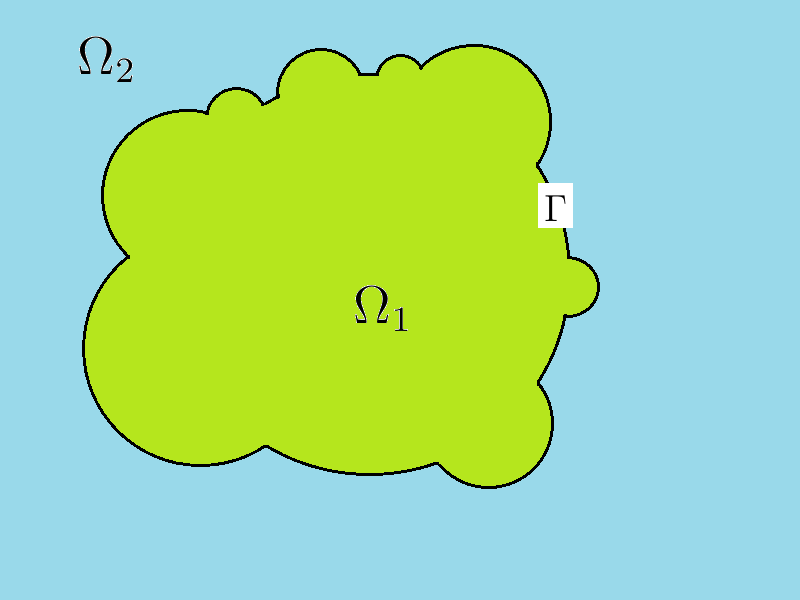
\includegraphics[width=0.3\linewidth]{\fpath pics/region0}}
\subfigure[截断后]{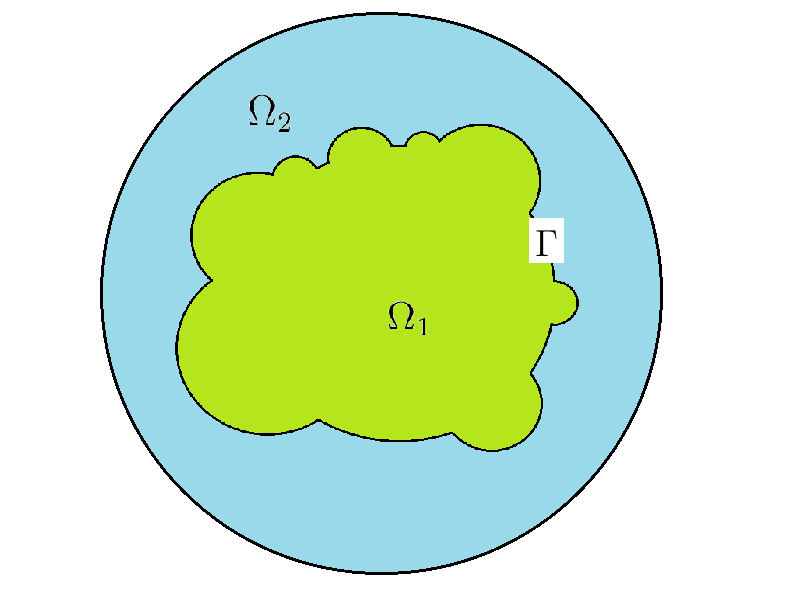
\includegraphics[width=0.3\linewidth]{\fpath pics/region1}}
\caption{无界区域截断示意图}
\label{regt}
\end{figure}

\BiSection{求解PB方程的有限差分法}{}

这里我们介绍一种简单的有限差分方法,用于求解PB方程并与深度学习方法进行对比。

在PB方程中,我们可以定义通量为$F(x) = \epsilon(x) \nabla u(x)$。尽管$\epsilon(x), \kappa(x)$和$u'(x)$可能是不连续的,根据边界条件我们可以得到,$u(x)$和$F(x)$连续且几乎处处可导。

考虑三维均匀网格上的数值解$u_{i,j,k}$,网格步长为$h$,我们有
$$ \frac{\partial u}{\partial x}(x_{i+\frac12}, y_{j}, z_{k}) \approx \delta_{x} u_{i+\frac12, j, k} $$
其中$x_{i+\frac12} = \frac{x_{i} + x_{i+1}}{2}$ 和 $\delta_{x} u_{i+\frac12, j, k} = \frac{u_{i+1, j, k} - u_{i, j, k}}{h}$。
这里我们可以定义数值通量为
$$ (F_1)_{i+\frac12, j, k} = \epsilon(x_{i+\frac12}, y_{j}, z_{k}) \; \delta_{x} u_{i+\frac12, j, k} $$
因此可以得到
$$ \frac{\partial F_1}{\partial x}(x_{i+\frac12}, y_{j}, z_{k}) \approx \delta_{x} (F_1)_{i, j, k} $$
这就是说
$$ \frac{\partial}{\partial x}(\epsilon \frac{\partial u}{\partial x}) (x_{i}, y_{j}, z_{k}) \approx \delta_{x} (\epsilon \delta_{x} u)_{i,j,k} $$
其中
$$ \delta_{x} (\epsilon \delta_{x} u)_{i,j,k} = \epsilon(x_{i+\frac12}, y_{j}, z_{k}) u_{i+1, j, k} - \epsilon(x_{i-\frac12}, y_{j}, z_{k}) u_{i-1, j, k} + (\epsilon(x_{i+\frac12}, y_{j}, z_{k}) + \epsilon(x_{i-\frac12}, y_{j}, z_{k})) u_{i, j, k} $$
在对其它方向进行类似的处理之后,我们可以得到最终的有限差分格式为
$$ -(\delta_{x} (\epsilon \delta_{x} u)_{i,j,k} + \delta_{y} (\epsilon \delta_{y} u)_{i,j,k} + \delta_{z} (\epsilon \delta_{z} u)_{i,j,k}) + \kappa(x_{i}, y_{j}, z_{k}) u_{i,j,k} = f(x_{i}, y_{j}, z_{k}) $$


\BiSection{具有几何奇异性的PB方程}{}

考虑到分子计算中的问题通常具有几何奇异性,我们构造具有几何奇异性的区域如下。首先选择一个中心在位于原点,半径为$0.5$的大球。在大球表面随机抽取20个点,以这些点为中心生成许多小球。小球的半径从$[0.1, 0.2]$中随机抽取。选取$\Omega_1$是这些小球和大球的并集。$\Omega_1$的形状如图\ref{region}所示。各个球之间的相交会产生几何奇异性,这对传统的有限元法和边界元法的网格生成以及精确求解提出了很大的挑战。

\begin{figure}[htbp]
\centering
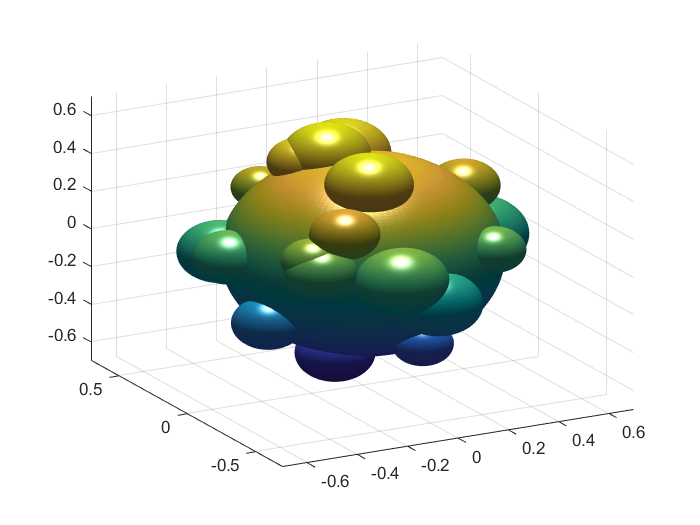
\includegraphics[width=0.4\linewidth]{\fpath pics/region3d}
\caption{具有几何奇异性的区域}
\label{region}
\end{figure}

我们在此区域上,首先考虑如下两个示例:

\textbf{示例 1:}方程的精确解表示为:
\begin{equation}
u(x) = \frac{e^{\sin \mu x_1 + \sin \mu x_2 + \sin \mu x_3}}{|x|^2 + 1} (|x|^2 - 1)
\end{equation}
方程的系数选取为
\begin{equation}
\mu = 15, \ \epsilon(x) = 1, \ \kappa(x) = 1 \ {\rm for}\ x\in\Omega_1, \ \epsilon(x) = 1, \kappa(x) = 5 \ {\rm for}\ x\in\Omega_2.
\end{equation}
方程的右端项由精确解生成。

求解区域被一个球心位于原点,半径为1的大球截断。在球面上,精确解满足对应的边界条件。

\textbf{示例 2:}方程中,右端项选取为
\begin{equation}
f(x) = \frac{e^{\sin \mu x_1 + \sin \mu x_2 + \sin \mu x_3}}{|x|^2 + 1} (|x|^2 - 1)
\end{equation}
方程的系数选取为
\begin{equation}
\mu = 20, \ \epsilon(x) = 1 \ {\rm for}\ x\in\Omega_1, \  \epsilon(x) = 80 \ {\rm for}\ x\in\Omega_2,\ \kappa(x) = 1.
\end{equation}
此时方程的精确解无法写出。在这种情况下,求解区域被立方体$[-1,1]^3$截断,参考解通过有限差分法(FDM)计算。在差分法中,我们选取了具有足够的精细的网格以确保精度。

在示例1中,在每个训练步,我们在区域$\Omega$内采样$5000$个点,在边界$\partial\Omega$上采样$4000$个点。在示例2中,我们对区域$\Omega$内的$6000$个点和边界$\partial\Omega$上的$3000$个点进行采样。需要注意的是,由于我们使用了Ritz方法,我们无需在界面$\Gamma$上采样,所有的跳跃边界条件都是自动满足的。

如图\ref{e14}所示。多尺度网络与普通的全连接网络相比,误差下降得更快。在两个示例中,多尺度网络都显示了很大的优势。
\begin{figure}[htbp]
\centering
\subfigure[示例1]{\includegraphics[width=0.35\linewidth]{\fpath E9P1}}
\subfigure[示例2]{\includegraphics[width=0.35\linewidth]{\fpath E9P2}}
\caption{不同网络结构在求解PB方程中的表现}
\label{e14}
\end{figure}

我们在图\ref{e9f}展示了示例2中,不同方法得到得近似解在横截面$x_1 = x_3 = 0$上的取值,包括FDM($h=0.02$)、normal(训练4000步)和Mscale(训练4000步)。普通的全连通网络在区域的内部给出了错误的解,而多尺度网络的结果和参考解相近。这些实例表明,相比于普通的全连接网络,多尺度网络求解复杂区域上的PB方程的速度更快,精度更高。

\begin{figure}[htbp]
\centering
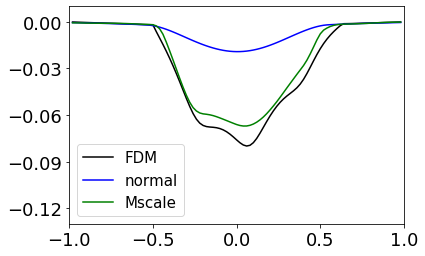
\includegraphics[width=0.35\linewidth]{\fpath exp14/M20E80_samp1}
\caption{示例2中不同方法得到的近似解在截面 $x_1 = x_3 = 0$上的图像}
\label{e9f}
\end{figure}

\BiSection{具有源项奇异性的PB方程}{}

在实际的生物分子中,电荷往往以点电荷的形式分布在分子内部,这就相当于方程中的右端项变为
\begin{equation}
f(x) = \sum_{k=1}^{K} q_k \delta(x - s_k)
\end{equation}
其中$\delta(x)$是Dirac函数,$q_k$和$\mathbf{s}_k$分别表示分子中点电荷的带电量和位置。我们假设核与分子界面之间的距离大于常量$R_0$。也就是说我们可以选取$\Omega_0=\{x:\exists k, | x-s_k|<R_0\}\subset\Omega_1$。在图\ref{region2}中,蓝色部分表示溶剂域$\Omega_2$,绿色部分表示生物分子区域$\Omega_1\setminus\Omega_0$,粉红色部分表示$\Omega_0$。这里$\Omega_0$是一些球的并集,其中已经包含了所有的点电荷。

\begin{figure}[htbp]
\centering
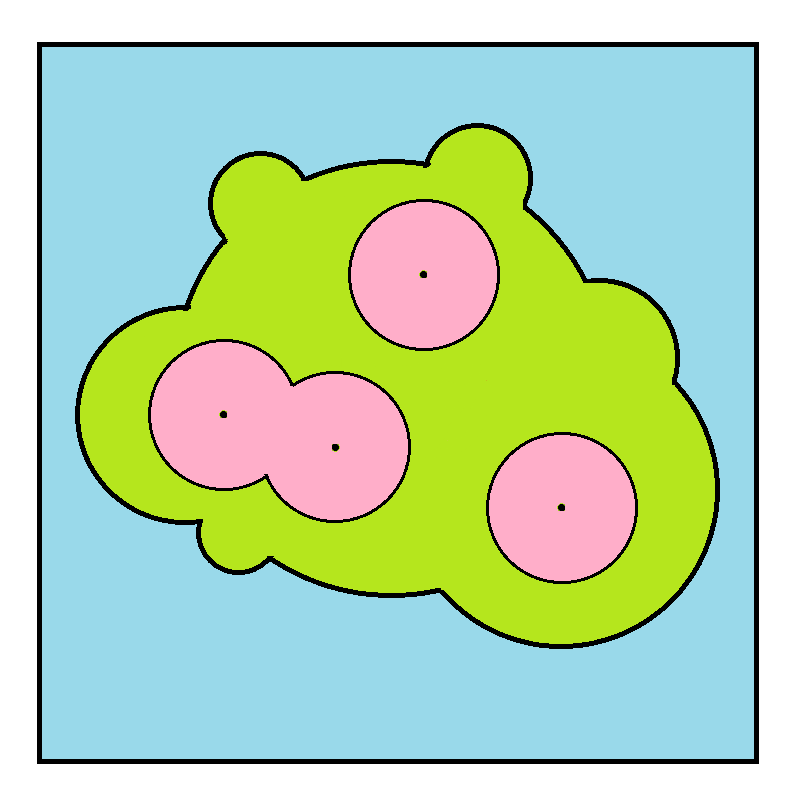
\includegraphics[width=0.25\linewidth]{\fpath pics/region2}
\caption{点电荷分布示意图}
\label{region2}
\end{figure}

这里我们给出一种克服源项奇异性的方法。我们首先定义
\begin{equation}
\bar{u}(x) = \sum_{k=1}^{K} q_k G(x - s_k) m(x - s_k)
\end{equation}
其中格林函数
\begin{equation}
G(x) = \frac{1}{4 \pi \epsilon_1} \frac{e^{-\frac{\kappa_1}{\sqrt{\epsilon_1}} |x|}}{|x|}
\end{equation}
截断函数
\begin{equation}
m(x) = \left\{
\begin{split}
1 - \left(\frac{|x|}{R_0}\right)^3 \left(4 - 3 \frac{|x|}{R_0} \right) &\quad |x| < R_0 \\
0 &\quad |x| > R_0
\end{split}
\right.
\end{equation}

通过以上定义,我们可以验证$\bar{u}(x)$满足
\begin{equation}
\begin{split}
-\Delta \bar{u}(x) + \kappa^2 \bar{u}(x) & = \sum_{k=1}^{K} q_k \delta(x - s_k) + \sum_{k=1}^{K} q_k F(|x - s_k|) \quad x \in \Omega_0 \\
\bar u= \frac{\partial \bar u}{\partial n} & = 0 \quad x \in \partial \Omega_0 \\
\bar{u}(x) & = 0 \quad x \in \Omega_0^c
\end{split}
\end{equation}

我们定义消除奇异性之后的解为
\begin{equation}
w(x) = u(x) - \bar{u}(x)  \chi_{\Omega_0}(x)
\end{equation}
奇异性之后的解满足这样一个没有奇异性的方程
\begin{equation}
\label{eqws}
- \epsilon(x) \triangle w(x) + \kappa^2(x) w(x)  = f(x) \chi_{\Omega_0}(x)
\end{equation}
其中
\begin{equation}
f(x) = -\sum_{k=1}^{K} q_k F(|x - s_k|)
\end{equation}
和
\begin{equation}
F(r) = \left\{
\begin{split}
\frac{3 \mathrm{e}^{-\frac{\kappa_1}{\sqrt{\epsilon_1}} r}}{\pi R_0^4} (2 R_0 - 3 r + 2 \frac{\kappa_1}{\sqrt{\epsilon_1}} r^2 - 2 R_0 \frac{\kappa_1}{\sqrt{\epsilon_1}} r) & \quad r < R_0\\
0 & \quad r > R_0
\end{split}
\right.
\end{equation}
这里我们只要求解消去奇异性之后的方程,就可以得到原方程的解了。

下面我们选取示例,验证多尺度网络对消去奇异性之后方程的求解能力。

\textbf{示例 1:}
这里我们选取大区域$\Omega = [-1,1]^3$,$\Omega_1$是一个中心位于原点,半径为$R = 0.7$的球。其它相关参数选择为
$$ s = (0,0,0), \quad q = 1, \quad R_0 = 0.5, \quad \epsilon(x) = 1 \ {\rm for}\ x\in\Omega_1, \ \epsilon(x) = 80 \ {\rm for}\ x\in\Omega_2,\ \kappa(x) = 0. $$

由于此时的区域不再具有几何奇异性,我们可以算出方程的精确解为
\begin{equation}
u(x) = \left\{
\begin{split}
\frac{1}{4\pi |x| \epsilon_1} - (\frac{1}{\epsilon_1} - \frac{1}{\epsilon_2}) \frac{1}{4\pi R} &\quad x\in\Omega_1 \\
\frac{1}{4\pi |x| \epsilon_2} &\quad x\in\Omega_2
\end{split}
\right.
\end{equation}
相应地,去掉奇异性的解为
\begin{equation}
w(x) = \left\{
\begin{split}
\frac{1}{4 \pi \epsilon_1 |x|} \left(\frac{|x|}{R_0}\right)^3 \left(4 - 3 \frac{|x|}{R_0} \right) - (\frac{1}{\epsilon_1} - \frac{1}{\epsilon_2}) \frac{1}{4\pi R} &\quad |x| < R_0 \\
\frac{1}{4\pi |x| \epsilon_1} - (\frac{1}{\epsilon_1} - \frac{1}{\epsilon_2}) \frac{1}{4\pi R} &\quad R_0 < |x| < R \\
\frac{1}{4\pi |x| \epsilon_2} &\quad |x| > R
\end{split}
\right.
\end{equation}

\textbf{示例 2:}
在第二个示例中,我们选择大区域$\Omega=[-1,1]^3$。区域$\Omega_1$构造如下。我们选择一个中心为原点,半径$0.7$的大球。在大球表面随机抽取20个点作为小球的中心。小球的半径从$[0.1, 0.3]$范围内的均匀分布中随机抽取。$\Omega_1$是这些球的并集。带有奇异性的源项构造为。每个电荷的位置在一个球心位于原点,半径$0.5$的球中随机选择,电荷量从$[-0.5,0.5]$范围内的均匀分布中随机抽样。我们选择$R_0=0.2$。如图\ref{reg},图中蓝色区域表示$\Omega_1$,在蓝色区域内的红色部分表示$\Omega_0$。
\begin{figure}[htbp]
\centering
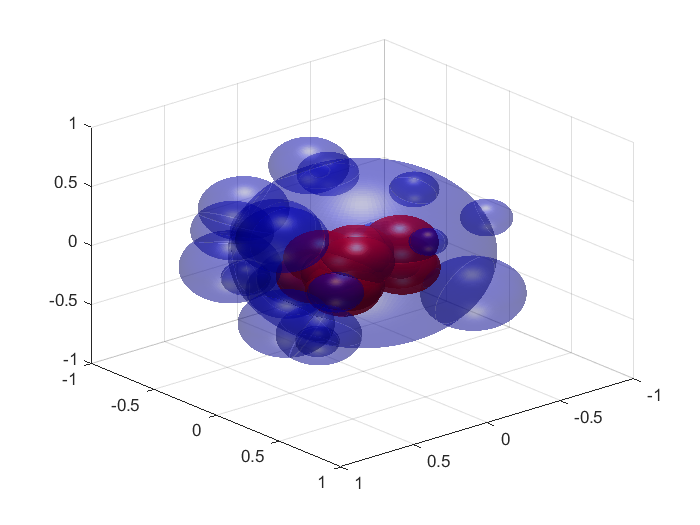
\includegraphics[width=0.45\linewidth]{\fpath pics/region4}
\caption{求解区域图像}
\label{reg}
\end{figure}

其它参数选择如下
$$ \epsilon(x) = 1 \ {\rm for}\ x\in\Omega_1 \ \epsilon(x) = 80 \ {\rm for}\ x\in\Omega_2 \ \kappa(x) = 0 $$
需要注意的是,示例2中同时具有几何奇异性和源项的奇异性,这给普通的数值方法带来了很大的挑战。这里我们无法得到精确解,参考解同样由FDM给出。

每步中我们随机在区域$[-1, 1]^d$内选取$5000$个均匀分布的积分点,在边界上生成$4000$个均匀分布的积分点。

\begin{figure}[htbp]
\centering
\subfigure[示例 1]{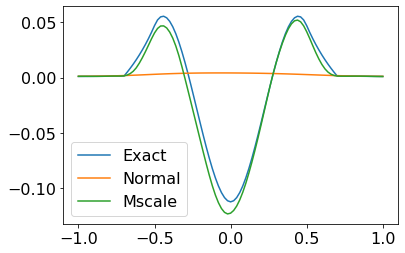
\includegraphics[width=0.35\linewidth]{\fpath expn/samp1}}
\subfigure[示例 2]{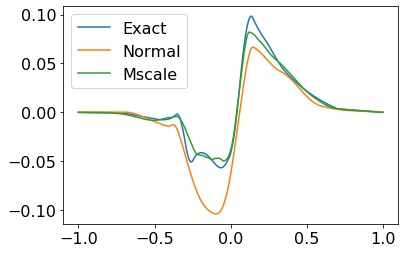
\includegraphics[width=0.35\linewidth]{\fpath expn/samp2}}
\caption{不同方法得到的近似解在截面 $x_2 = x_3 = 0$上的图像}
\label{ens}
\end{figure}

在示例1中,方程具有源项奇异性,我们测试的网络结构如下:
\begin{enumerate}
\item 规模为\textbf{1-1000-1000-500-1}的全连接网络。(Normal)
\item \textbf{5}个规模为\textbf{1-200-200-100-1}的多尺度网络,系数为$\{1,2,4,8,16\}$。(Mscale)
\end{enumerate}

在示例2中,方程同时具有几何奇异性和源项奇异性,因此我们需要更多的神经元,使网络具有更强的逼近能力。这里测试的网络结构如下:
\begin{enumerate}
\item 规模为\textbf{1-1500-1000-1000-500-1}的全连接网络。(Normal)
\item \textbf{5}个规模为\textbf{1-300-200-200-100-1}的多尺度网络,系数为$\{1,2,4,8,16\}$。(Mscale)
\end{enumerate}

通过三种方法:FDM($h=0.01$)、normal(训练$10000$步)和Mscale(训练$10000$步)得到的截面上的数值解如图\ref{ens}所示。正常全连通网络的输出不能很好地捕捉精确解中的峰值,而多尺度网络得到了更加精确的结果。
